\subsection{Descripción del problema.}
En esta sección vamos a tratar el problema List Coloring para grafos, que tienen la particularidad que que cada nodo tiene una lista de colores que puede ser a los sumo de tamaño C, osea:
\begin{center}
$(\forall v \in V(G)) \neg \emptyset(coloresOriginales(v)) \land ((\forall c \in coloresOriginales(v) ) 0\leq c <C)$ donde $1\leq C$
\end{center}
El grafo posee N nodos, todos los nodos están enumerados de $0$ hasta $N-1$. También no hay dos nodos distinto que tengan el mismo Id, mas formalmente : \newline
\begin{center}
	$(\forall i \in [0..N-2])Id(Nodo_i) \neq Id(Nodo_j)$
\end{center}
También tenemos M arista,  donde $M\geq 0$ \newline 


\subsection{Desarrollo de la idea de resolución}
\vspace*{0.3cm}
%\textbf{completar!}
Para la resolución de este problema utilizamos a tres técnicas algorítmicas diferentes, las cuales enumeramos de la siguiente manera:
 \begin{itemize}
	\item[1.] Algoritmo exacto usando backtracking con podas(es eficiente en varios casos), tiene mas podas.
	Una de las podas es fijarse si el grafo es 2-ListColoring. Si los es aplicamos el algoritmo explicado en el ejercicio. \newline
	La otra poda es verificar si se puede pintar el nodo actual con uno de los colores de su lista, esta verificación se hace revisando todos los nodos vecinos para ver de que color están pintados(también puede pasar que no este pintado). Si se puede pinto el nodo y hago la llamada recursiva al próximo nodo a procesar. este proceso se hace con cada color de su lista de colores posibles.
	\item[2.] backtraking sin podas, esto es que tiene una poda mínima, osea es parecido al backtraking pero no utiliza ningún tipo de poda(Es bastante ineficiente). Con poda mínima me refiero a que el algoritmo no se ejecuta mas si encuentra una solución.
	La idea de este algoritmo es pintar todo el grafo, y una vez terminado de pintar verificar si el grafo es List Coloring. En el caso en que no es List Coloring, pinto los nodos utilizando otro color de su lista de colores posibles para pintar el ese nodo. 
	 
	\item[3.] Sin ninguna poda, osea fuerza bruta pruebas todos los casos posibles. Continua ejecutando a pesar de ya haber encontrado un coloreo valido. Por esto este algoritmo es menos eficiente, dado que no realiza ni una poda.\newline
	La idea es arrancar a pintar el nodo_0 (Nodo que tiene el id 0) primero con el primer color de su lista, para ese color pintamos luego el nodo_1 con cada uno de sus respectivos colores.. etc. De esta manera obtenemos todas las posibles formas de pintar el grafo(soluciones y no soluciones) a partir del primer color del nodo_0, nos guardamos el valor de la solución en una colección(vector,conjunto,lista, etc)... ahora probamos con el segundo color de la lista de colores del nodo_0 ... y así sucesivamente. \newline
	Después de todo esto, recién devolvemos si es solución o no.  Como se ve es bastante ineficiente esta forma de resolver el problema $ListColoring$ (ver algoritmo \proc{tieneColoreoSinNingunaPodas} abajo).
	\item[4.] Cantidad de conflictos menor, tambien fuerza bruta. 
	La idea general de este algoritmo es pintar el grafo(pintadas validas o no validas como solución). Luego a lo ultimo evaluar si el grafo esta pintado correctamente. \newline
	Voy a definir como cantidad de conflictos a la cantidad de nodos vecinos que tienen el mismo color que el nodo actual que se esta revisando.
	Esta evalución se hace contando la cantidad de conflictos que tiene un nodo del grafo. Si todos los nodos del grafo tienen cantidad de conflictos igual a 0,entonces esto implica que es solución.  
 \end{itemize}

%\begin{figure}[htb]
%  \begin{center}
%      \includegraphics[scale=0.25]{imagenes/ejemplo.jpg}
%  \end{center}
%  \caption{ejemplo}
%\end{figure}



%\newpage
\subsection{Ánalisis de complejidad Y Pseudocódigo del backtraking.}
\vspace*{0.3cm}
%\textbf{completar!}

\subsubsection{Con podas} 

Para explicar la complejidad del algoritmo vamos a recurrir al pseudocódigo en ciertas secciones de la explicación. Este algoritmo usamos técnica de backtracking con cierto tipo de podas podas.
Para representar el grafo utilizaremos \underline{listas de adyacencia}. 

Cuando arranca algoritmo, empieza tomando el primer nodo de la lista de adyacencia (TIENECOLOREOPODAS linea 1). Luego el algoritmo empieza a realizar el backtracking propiamente dicho.\newline
Ahora ingresamos a la funcion TIENECOLOREOAUXPODAS: \newline 
Primero examinamos si todos los nodos tienen a lo sumo 2 colores(linea 5), ahí aplicamos 2-ListColoring de complejidad polinomial .\newline Sino tomamos el nodo actual y examinamos si se puede pintar con alguno de los colores disponibles para el, esto puede tomar $O(C)$ iteraciones en el peor caso, pues examínanos todos los colores posibles de su lista de colores disponibles(Ver linea 8). Dentro de de este ciclo examinamos si se puede pintar el nodoActual, para eso debemos explorar todos sus nodos vecinos(linea 9), que en el peor caso es $O(N-1)$ pues podría tener de vecinos a todos los nodos del grafo.
También borro el color de la lista de mis colores disponibles(linea 11), esto a los sumo me cuesta $O(C)$.
Por ultimo tengo que hacer una recursión hacia la misma función(linea 13), con la característica que el nodo a procesar sera el siguiente del grafo modelado con listas de adyacencias, esto ultimo tiene complejidad $T(N-1)$. Y esto se puede repetir C veces como dije al principio de este párrafo.\newline

De este analisis se desprende la siguiente función de recurrencia, con la cual trataremos de calcular la complejidad estimada. \newline
$T(N)=C*T(N-1)+C^{2}+C*(N-1)$
Podríamos hacerles unos pequeños calculos para obtener la complejidad. Como C es constante podríamos sacarlos de la ecuación de recurrencia. También de la parte (N-1) podría tomar directamente N, dado que el -1 no aporta demasiado a la complejidad, pues tiene la pinta de ser Exponencial.
 
\begin{equation*}
T(N) = \left\lbrace
\begin{array}{c}
		1 \ \ \ \ \ \ \ \ \ \ \ si \ \ \ \   N = 0 \\
		C*T(N-1)+N  \  \ \ \  \ si \ \ \ \  N>0 \\
\end{array}
\right.
\end{equation*}

Haciendo las reducciones pertinentes nos queda una complejidad de $O(C^{N}*N^{2})$
%$T(N)=c*T(N-1)+C^{2}+C*(N-1)$
%Vamos a tomar a C como una constante, podriamos simplificar aun mas la ecuacion de recurencia
%$T(N)=C*((N-1)+C+T(N-1))=C*T(N-1)+C^{2}+C*(N-1)=$
%$T(N)=C(C*T(N-2)+C^{2}+C*(N-2))+C^{2}+C*(N-1)=C^{2}T(N-2)+C^{3}+C^{2}*(N-2)+C^{2}+C*(N-1)$
%$=C^{2}T(N-2)$	

\begin{codebox}
\Procname{$\proc{tieneColoreoPodas}(Arreglo: nodosGrafo)$ $\longrightarrow res:Bool$}
	\li \Return  tieneColoreoAuxPodas(nodoGrafo,0)%$\id{solucion}$
\end{codebox}


\begin{codebox}
\Procname{$\proc{tieneColoreoAuxPodas}(Arreglo: nodosGrafo, Nat: nunNodo)$ $\longrightarrow res:Bool$}
	\li \Comment{Caso base 1: Ya Visitamos todos los nodos}
	\li \If $nodoGrafo  [ nunNodo ] = tamanio(NodoGrafo)$; 
	\li		\Then \Return $\id{True}$; \Comment{Caso base: $O(1)$}
		\End   
	\li \Comment{Caso base 2} 
	\li \If todos los nodos tienen como maximo 2 colores pisibles para usar; 
	\li 	\Then \Return $\id{aplico 2-list Coloring}$; \Comment{ $O(Polinomial)$} 
		\End
	\li $Nodo$ $nodoActual \leftarrow nodoGrafo [ nunNodo ]$;
	\li	\For $Nat$ color $:$ \To $ coloresPosibles(nodoActual); $; \Comment{$T(n)=C*(O(N-1)+O(C)+1+T(N-1))$} \Do 
	\li		\If $sePuedePintar(nodosGrafo, numNodo, color)$; \Comment{ .$O(N-1)= O(N)$.Ver aclaraciones abajo}
	\li			\Then $ pinto(nodoActual, color)$;	\Comment{O(1)}
	\li				  $ BorrarColor(nodoActual, color)$; \Comment{$O(C)$}
	\li 		\Comment{Recursion}
	\li			\If $ tieneColoreoAuxPodas(nodosGrafo, numNodo+1)$ \Comment{$T(N-1)$}
	\li				\Then Restauro ColoresOriginales de nodoActual; \Comment{ $O(C)$}		
	\li					\Return $\id{True}$;
				\End
			\End
		\End
	\li \Comment{En caso de que ninguno de los colores sirva para ese nodoActual, retornamos falso}	
	\li Restauro ColoresOriginales de nodoActual;\Comment{$O(C)$}
	\li \Return $\id{False}$;	
\end{codebox}

\begin{itemize}
    \item Algunas aclaraciones sobre el pseudocodigo.
		\begin{description}
			\item[Linea 8:] Itera la lista de colores posibles pertenecientes a ese nodoActual. En el peor caso podria iterar $C$ veces($C=\#coloresMaximos$). 
			\item[Linea 9:] $O(N-1) = O(N)$, pues para saber si se puede pintar deberia revisar a lo mucho N-1 nodos vecinos. Está es una poda que mejora el rendimiento nuestro algoritmo
			\item[Linea 10] Pintar es $O(1)$ pues es solo asignar un numero al atributo $Color$ del nodoActual.
			\item[Linea 12:] Borra el $color$ de la lista de ColoresPosibles hasta ese momento para colorear el nodoActual.
		\end{description}
\end{itemize}

\begin{codebox}
\Procname{$\proc{sePuedePintar}(Arreglo: nodosGrafo, Nat: nunNodo, Nat: color)$ $\longrightarrow res:Bool$}
	\li \Comment{indica si se puede pintar de ese color este nodoActual,}
	\li \Comment{es decir si todos los sucesores tienen otro color(no hay conflictos)}
	\li $Nodo$ $nodoActual \leftarrow nodoGrafo [ nunNodo ]$;
	\li	\For $Nodo$ sucesor $:$ \To $ sucesores(nodoActual); $; \Comment{como mucho itera $N-1$ veces($N=\#Nodos$)} \Do 
	\li		\If $ tieneColor(nodoActual) \land Color(sucesor) = color$; \Comment{ $O(1)$}	
	\li		\Then \Return $\id{False}$;
			\End
		\End	   
	\li \Return $\id{True}$;	
\end{codebox}

\subsubsection{Sin muchas podas} 

\vspace*{0.3cm}
El Analisisis de complejidad de este ejercicio es similar al anterior.
Cuando ejecutamos el algoritmo, siempre empieza haciendo la recursion a partir del primer nodo. Y es ahi donde me pongo a analisar la complejidad, osea mirando el algoritmo $TieneColoreoAuxSinPodas$ este algoritmo. \newline
Si estamos en el caso base, tenemos dos ciclos anidados como podemos ver(linea 3 a linea 7), por los tanto tenemos una complejidad de $O(N*(N-1))$. 
Pues  primero recorremos todos los nodos esto es $O(N)$ y para cada nodo recorremos sus sucesores(en peor caso es N-1), en total tenemos $O(N^2)$. \newline
Si no estamos en el caso base, nos toca ejecutar las lineas restante del algoritmo(linea 10 a 17).\newline
Tenemos un ciclo (lineas 11 a 15)que itera a los sumo C-veces(pues a lo sumo hay C colores en un nodo), y dento del ciclo tenemos la recursion hacia la misma funcion(linea 14), por lo tanto la complejidad de esto es: O(C)*T(N-1).\newline
Haciendo un cambio de variables, sabiendo que en este caso recorrer el arreglo empezando del  ultimo elemento hacia el primer elemento es lo mismo, la ecuación de recurrencia me quedaria así.

\begin{equation*}
T(N) = \left\lbrace
\begin{array}{c}
		N^2 \ \ \ \ \ \ \ \ \ \ \ si \ \ \ \   N = 1 \\
		$C*T(N-1)$  \  \ \ \  \ si \ \ \ \  N>1 \\
\end{array}
\right.
\end{equation*} 

Haciendo reducciones, se puede desmostrar que nuestro algoritmo es exponencial. Cuya complejidad es exactamente $O(C^N + N^2) = O(C^N)$.

\begin{codebox}
\Procname{$\proc{tieneColoreoSinPodas}(Arreglo: nodosGrafo)$ $\longrightarrow res:Bool$}
	\li \Return  $tieneColoreoAuxSinPodas(nodoGrafo,0)$%$\id{solucion}$
\end{codebox}

\begin{codebox}
\Procname{$\proc{tieneColoreoAuxSinPodas}(Arreglo: nodosGrafo, Nat: nunNodo)$ $\longrightarrow res:Bool$}
	\li \Comment{Caso base 1: Ya Visitamos todos los nodos}
	\li \If $nodoGrafo  [ nunNodo ] = tamanio(NodoGrafo)$; 
			\Then 
	\li			\For $Nodo:$ $nodoActual$ $:$ \To $ nodosGrafo; $; \Comment{} \Do
	\li				$Nat: colorAcutal \leftarrow obtenerColor(nodoActual)$;	
	\li				\For $Nodo:$ $sucesor $:$ \To $ $Sucesores(nodoActual); $\Do
	\li					\If $ color(sucesor) = colorActual$ 
	\li						\Then \Return $\id{False}$;
						\End
					\End
	\li
				\End
	\li		\Return $\id{True}$; \Comment{Caso base: $O(1)$}
		\End 	 
	\li $Nodo$ $nodoActual \leftarrow nodoGrafo [ nunNodo ]$;
	\li	\For $Nat$ color $:$ \To $ coloresPosibles(nodoActual); $; \Comment{} \Do 
	\li			$ pinto(nodoActual, color)$;	\Comment{O(1)}
	\li 		\Comment{Recursion}
	\li			\If $ tieneColoreoAuxSinPodas(nodosGrafo, numNodo+1)$ \Comment{$T(n-1)$}
	\li					\Return $\id{True}$;
				\End
		\End
	\li \Comment{En caso de que ninguno de los colores sirva para ese nodoActual, retornamos falso}	
	\li \Return $\id{False}$;	
\end{codebox}


\begin{itemize}
    \item Algunas aclaraciones sobre el pseudocodigo.
		\begin{description}
			\item[Linea 15:] Aca hay una minima poda, que es quedarse con la solucion si ya la encontro.
		\end{description}
\end{itemize}




\subsubsection{Fuerza bruta 1} 
\vspace*{0.3cm}
Como podemos obserbar en el pseudocódigo de abajo, la primera llamada se hace es a la función \proc{tieneColoreoSinNingunaPodas}, que es la que resuelve el problema de $ListColoring$. A su vez la función antes nombrada llama a \proc{tieneColoreoAuxSinNingunaPodas} que es la función que se va llamar recursivamente empezando desde el nodo numero Cero, y desde aquí vamos a analizar la complejidad temporal. \newline

1) Analisis de complejidad del caso base(linea 2 a 11 pseudocódigo): LLegamos al caso base cuando ya no hay mas nodos por recorrer en las llamadas recursivas a \proc{tieneColoreoAuxSinNingunaPodas}. La complejidad de este caso base es $N*(N-1)$, pues tengo dos ciclos anidados: 
\begin{itemize}
	\item El ciclo mayor recorre todos los nodos(osea $N$ iteraciones), para obtener el color del cual esta pintado (linea 3) el nodoActual.
	\begin{itemize}
		\item El ciclo menor  recorre todos los nodos sucesores de dicho nodo, osea $N-1$ interaciones en el peor caso, pues el grafo puede ser completo(Tener a todos los nodos son vecinos). Esto lo hace para saber si el coloreo de los nodos es solución o no (devuelve TRUE O FALSE). 
	\end{itemize}  
\end{itemize}

2)Analisis del caso recursivo(linea 12 a 25): En este caso para cada nodo nos cremas un vector de booleanos llamando \underline{\textsl{SonSolucionesPosibles}}, que tiene tamaño colores posibles con que se puede pintar el nodoActual, que en peor caso es $O(C)$(ver linea 14), pues es la cantidad máxima de colores que puede tener. Luego inicializamos la variable \underline{\textit{ind}} en cero, la cual nos sirve para hacer referencia una posición del  vector \textsl{SonSolucionesPosibles}. \newline
A partir de la linea 16  hasta la 21, tenemos un ciclo en cual itera todos los colores posibles que se pueden usar para pintar el nodo en ese instante de la ejecución del algoritmo, en peor caso es $O(C)$. Una vez dentro del ciclo pinto el nodo (linea 17)y hago las las llamandas recursivas a la funcion \proc{tieneColoreoAuxSinNingunaPodas} pasando como argumentos el grafo y el próximo nodo a revisar, la complejidad es $O(T(N-1))$. Dependiendo si la respuesta que me da la funcion \proc{tieneColoreoAuxSinNingunaPodas} es TRUE o FALSE y lo copio en la posición del vector $SonSolucionesPosibles[ind]$(complejidad $O(1)$).
En total el ciclo Tiene complejidad $O(C*(T(N-1)))$. \newline
Por ultimo en las lineas 22 a 24, verificamos si hay solución al problema, esto se hace recorriendo todo el vector  de boleanos    $SonSolucionesPosibles$ encontrando algun TRUE. Esto nos demanda C iteraciones en el peor caso, complejidad es $O(C)$.\newline
En total la complejidad del caso recursivo es $O(C+CT(N-1)+C)=O(CT(N-1)+2C)$. \newline

Haciendo un cambio de variables, sabiendo que en este caso recorrer el arreglo empezando del  ultimo elemento hacia el primer elemento es lo mismo, la ecuación de recurrencia me quedaria así.
  
\begin{equation*}
T(N) = \left\lbrace
\begin{array}{c}
		N*(N-1) \ \ \ \ \ \ \ \ \ \ \ si \ \ \ \   N = 1 \\
		$C*T(N-1)+2*C$  \  \ \ \  \ si \ \ \ \  N>1 \\
\end{array}
\right.
\end{equation*} 

Reduciendo: 
\begin{center}
$C*T(N-1)+2C = C*(C*T(N-2)+2C)+2C= ...= C^N*(N*(N-1)+N)+2*\sum_{i=1}^{N}C^i=C^N*N^2+2*\sum_{i=1}^{N}C^i$ \newline
$C*T(N-1)+2C = C^N*N^2+2*(C^{N+1}-C)/C-1 $
%\end{center}
\newline
Calculo auxiliar:  \newline
%\begin{center}
\newline
Luego todo esto nos queda \newline
$C*T(N-1)+2C = C^N*N^2+2*(C^{N+1}-C)/C-1 $
\end{center}
En concluición la complejidad nos queda exponencial en el caso en que C es fijo. \newline 
\begin{center} 
$O(C^N*N^2+2*(C^{N+1}-C)/C-1)=O(C^N*N^2)$
\end{center}
		
\begin{codebox}
\Procname{$\proc{tieneColoreoSinNingunaPodas}(Arreglo: nodosGrafo)$ $\longrightarrow res:Bool$}
	\li $Array<Nat>$ $coloresSinNingunaPoda \leftarrow NewArray[tamanio(nodosGrafo)]$; \Comment{$O(N)$} 
	\li \Return  $tieneColoreoAuxSinPodas(nodoGrafo,0)$%$\id{solucion}$
\end{codebox}

\begin{codebox}
\Procname{$\proc{tieneColoreoAuxSinNingunaPodas}(Arreglo: nodosGrafo, Nat: nunNodo)$ $\longrightarrow res:Bool$}
	\li \Comment{Caso base 1: Ya Visitamos todos los nodos}
	\li \If $nodoGrafo  [ nunNodo ] = tamanio(NodoGrafo)$; 
			\Then 
	\li			\For $Nodo:$ $nodoActual$ $:$ \To $ nodosGrafo; $; \Comment{} \Do
	\li				$Nat: colorAcutal \leftarrow obtenerColor(nodoActual)$; \hfill{$O(1)$}	
	\li				\For $Nodo:$ $sucesor $:$ \To $ $Sucesores(nodoActual); $\Do
	\li					\If $ color(sucesor) = colorActual$ 
	\li						\Then \Return $\id{False}$;
						\End
					\End
	\li
				\End
				\li	\For $Nat$ i $:$ \To $ tamanio(coloresSinNingunaPoda); $; \Comment{$O(N)$} \Do 
				\li			$ coloresSinNingunaPoda[i] \leftarrow nodosGrafo[i].getColor();$;	\Comment{O(1)}
					\End				
	\li		\Return $\id{True}$; \Comment{Caso base: $O(1)$}
		\End 	 
	\li $Nodo$ $nodoActual \leftarrow nodosGrafo[nunNodo]$
	\li // el arreglo de de abajo esta inicialido todo en false
	\li $Array<booleano>$ $SonSolucionesPosibles$ $\leftarrow$ $array[tamanio(coloresPosibles(nodoActual))]$;	
	\li $Nat $ $ind \leftarrow 0$;
	\li	\For $Nat$ color $:$ \To $ coloresPosibles(nodoActual); $; \Comment{} \Do 
	\li			$ pinto(nodoActual, color)$;	\Comment{O(1)}
	\li 		\Comment{Recursion}
	\li			\If $ tieneColoreoAuxSinNingunaPodas(nodosGrafo, numNodo+1)$ \Comment{$T(n-1)$}
	\li				\Then	$sonSolucionesPosibles[ind] \leftarrow True$;
	\li				\Else 	$sonSolucionesPosibles[ind] \leftarrow False$;		
				\End
		\End
	\li $res \leftarrow false$	
	\li \For $Nat$ sp $:$ \To $ solucionesPosibles; $; \Comment{} \Do
	\li		$res \leftarrow res \lor sp $;	
		\End	
	\li \Return $\id{res}$;	
\end{codebox}

\subsubsection{Fuerza bruta 2} 


Recordamos que la función que me dice si el grafo se puede colorear es $\proc{tieneColoreoCantidadConflictosOptima}$. Esta funcion a su vez llama a la función  $\proc{tieneColoreoCantidadConflictosOptimaAux}$ que es en la que aplicamos la recursion, es de de aqui que vamos a empezar a analizar la complejidad. \newline 

En la funcion $\proc{tieneColoreoCantidadConflictosOptimaAux}$ podemos obserbar que el caso base que tiene una complejidad $2N^2 -N$ (linea de 2 a 7). Esto se debe a que en la linea 3 tenemos un llamado a la funcion \proc{CalcularCantidadDeConflictos} que tiene una complejidad  $N*(N-1)$ pues tiene dos ciclos anidados. El primer itera los N nodos y el segundo itera la cantidad de vecinos del nodo, que en peor caso tiene N-1 vecinos. Luego en la linea 6 a 7 tenemos un ciclo for que itera N veces. En definiva esto nos da un total de :  
\begin{center}  $ N*((N-1)+N)= 2*N^2 - N $\end{center}


El caso recursivo (lineas de 9 a 11): \newline
Tenemos un for anidado el cual itera los colores posibles del nodo actual, que en pero caso es $C$(pues el grafo puede ser completo). Una vez dentro del for tenemos la llamada recursiva(linea 11)y asignaciones que son $O(1)$. En total el caso recusivo tiene una complejidad $O(C*T(N-1))$. \newline

Haciendo un cambio de variables, sabiendo que en este caso recorrer el arreglo empezando del  ultimo elemento hacia el primer elemento es lo mismo, la ecuación de recurrencia me quedaria así.
  
\begin{equation*}
T(N) = \left\lbrace
\begin{array}{c}
		2*N^2 - N \ \ \ \ \ \ \ \ \ \ \ si \ \ \ \   N = 1 \\
		$C*T(N-1)$  \  \ \ \  \ si \ \ \ \  N>1 \\
\end{array}
\right.
\end{equation*}
 
Reduciendo: 
\begin{center}
$C*T(N-1) = C*C*T(N-2)= ...= C^N*(N^2-N)) $ \newline
\end{center}

Luego la complejidad total del algoritmo Fuerza Bruta 2 es : $O(C^N * (2N^2-N)) = O(2*C^N*N^2)$

\vspace*{0.3cm}
\begin{codebox}
	\li $Nat$  $minimaCantidadConflictos \leftarrow \infty$; // variable global que uso en las funciones de abajo
\end{codebox}

\begin{codebox}
\Procname{$\proc{tieneColoreoCantidadConflictosOptima}(Arreglo: nodosGrafo)$ $\longrightarrow res:Bool$}
	\li $cantidadConflictosOptimaAux(nodosGrafo,0)$;
	\li \Return  $minimaCantidadConflictos=0$%$\id{solucion}$
\end{codebox}

\begin{codebox}
\Procname{$\proc{cantidadConflictosOptimaAux}(Arreglo: nodosGrafo, Nat: nunNodo)$}
	\li \Comment{Caso base 1: Ya Visitamos todos los nodos}
	\li \If $nodoGrafo  [ nunNodo ] = tamanio(NodoGrafo)$; 
			\Then
	\li		$Nat$ $cantConflic \leftarrow calcularCantidadConflictos(nodosGrafo)$;
	\li 	\If $(cantConflic<minimaCantidadConflictos)$
	\li			\Then $minimaCantidadConflictos \leftarrow cantConflic$;
	\li				\For $Nat:$ $i \leftarrow 0 $:$ \To $ $i<tamanio(nodosGrafo); $\Do
	\li					$coloresOptimos[i] \leftarrow color(nodosGrafo[i])$;
					\End
			\End
		\End 				
 
	\li $Nodo$ $nodoActual \leftarrow nodosGrafo[nunNodo]$
	\li	\For $Nat$ color $:$ \To $ coloresPosibles(nodoActual); $; \Comment{} \Do 
	\li			$ pinto(nodoActual, color)$;	\Comment{O(1)}
	\li			$cantidadConflictosOptimaAux(nodosGrafo,0+1)$;
		\End
	\li FinFuntion	
\end{codebox}


\begin{codebox}
\Procname{$\proc{calcularCantidadConflictos}(Arreglo: nodosGrafo) \longrightarrow res :  Nat$}
	\li $Nat$ $cantConflictos \leftarrow 0$;
	\li	\For $Nodo$ nodoActual $:$ \To $ nodosGrafo; $; \Comment{} \Do
	\li		$ Nat$ $colorActual \leftarrow colorDeNodo(nodoActual)$;
	\li			\For $Nodot$ sucesor $:$ \To $ sucesores(nodoActual); $; \Comment{} \Do 
	\li				\If$(tieneColor(sucesor)$ $\land$ $dameColor(sucesor) = colorActual)$ \Then $cantConflictos++$;
					\End
				\End		 
		\End
	\li \Return  $cantConflictos/2$;%$\id{solucion}$
\end{codebox}

\begin{codebox}
\Procname{$\proc{cantidadConflictosOptima}(Arreglo: nodosGrafo)$}
	\li $cantidadConflictosOptimaAux(nodosGrafo,0)$;
	\li FinFuntion;
\end{codebox}



%\subsection{Justificación de la resolución y demostración de correctitud.}

%\vspace*{0.3cm}

%\textbf{completar!}



%\newpage
%\subsection{Análisis de complejidad.}

%\vspace*{0.3cm}

%%\textbf{completar!}
	
\newpage
\subsection{Experimentación y gráficos.}
En los siguientes experimentos vamos a tener muy encuenta dos resultados posibles del algoritmo, con esto nos referimos a los casos en que se puede colorear y a los casos en que no se puede colorear. \newline
Como la complejidad no depende de M. Decidimos que vamos a hacer los experimento respecto a las variables a N y C.
\vspace*{0.3cm}

%\subsubsection{Test2: C Fijo}
%En esta parte experimentaremos con los algoritmos 1 y 2 ( osea con podas y sin podas). Para ello fijaremos C, y usaremos grafos densos....... ME VOY A DORMIR CONTINUO CUANDO ME LEVANTE...


\vspace*{0.3cm}
\subsubsection{Test 1: C Fijo y el algoritmo encuentra la solución}


Para este test lo que hicimos fue dejar fijo $C = 7$, y variar la cantidad de nodos N desde 2 hasta 15 .\newline
La toma de tiempos se hará en milisegundo, tal como se indica en los gráficos. \newline
Los grafos que usaremos para esta experimentación seran densos, es decir que tendrán una gran cantidad de aristas por nodo. Como mucho el grafo podrá ser completo y otras veces maximal completo(osea le faltan muy pocas arista para llegar a ser completo).
Cada nodo tendrá una lista de colores, nos encargamos de distribuir la lista de colores de cada nodo de tal manera que el algoritmo tenga que hace backtraking  muchas veces.

\begin{figure}[htb]
  \begin{center}
      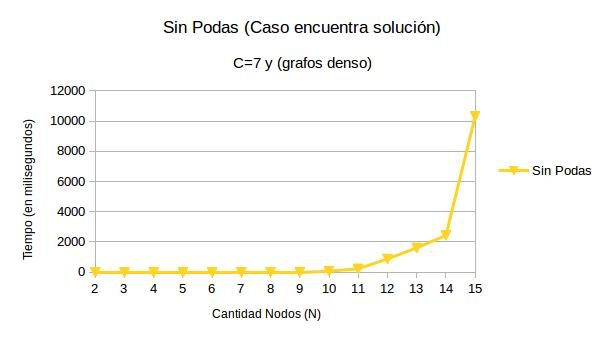
\includegraphics[scale=0.60]{imagenes/imgEjercicio2/SinPodas-solucion}
  \end{center}
  \caption{Tiempos caso en que hay solución}
\end{figure}

 \begin{figure}
 \centering
  \subfloat[Encuentra solución]{
   \label{Fuerz brut 1}
    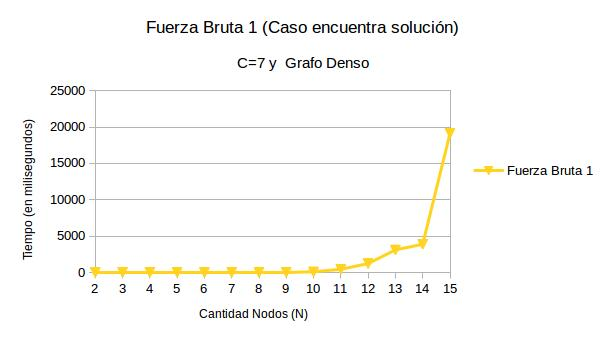
\includegraphics[width=0.55\textwidth]{imagenes/imgEjercicio2/FB1-solucion}}
  \subfloat[Encuentra solución]{
   \label{Fuerz brut 2}
    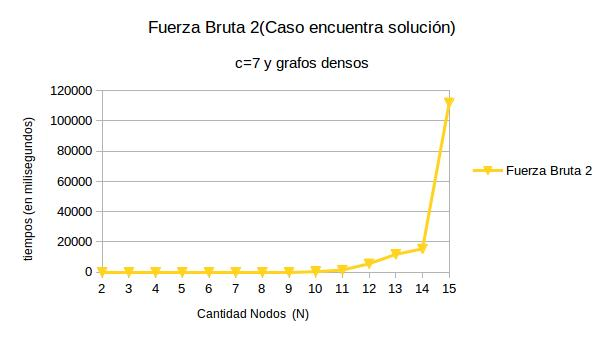
\includegraphics[width=0.55\textwidth]{imagenes/imgEjercicio2/FB2-solucion}}
 \caption{Tiempos caso en que hay solución}
 \label{tiempos}
\end{figure}

Como vemos nuestro algoritmo tiende a comportarse exponencialmente en los graficos. 
Ahora en el siguiente grafico veremos la comparación  entre los algoritmos.

\begin{figure}[htb]
  \begin{center}
      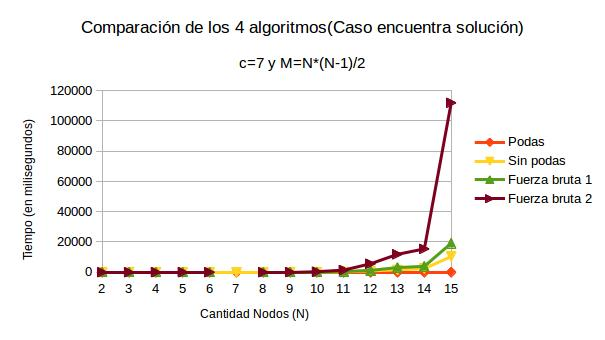
\includegraphics[scale=0.60]{imagenes/imgEjercicio2/CA4Solucion.jpg}
  \end{center}
  \caption{Comparacion de los tiempos}
\end{figure}

Como se ve en el grafico, los algoritmos menos eficiente son los de  \textbf{Fuerza bruta 1} y \textbf{Fuerza bruta 2} en comparación con las  versiones \textbf{Sin podas} y con \textbf{podas}. \newline
 
Cabe destacar que la versión mas eficiente es la version con \textbf{Podas} como se puede apreciar en el gráfico. 
 

\vspace*{0.3cm}

\subsubsection{Test 2: C fijo y el algoritmo no encuentra solución}

En este experimento analizaremos los casos en que  el algoritmo no encuentra la solución. Para esto fijaremos los la cantidad de colores C=7 y los grafos  que manejaremos serán completos. También colocaremos la lista de colores para cada grafo de manera tal que el algoritmo haga la mayor cantidad de bactrakings posibles.   



\begin{figure}[htb]
  \begin{center}
      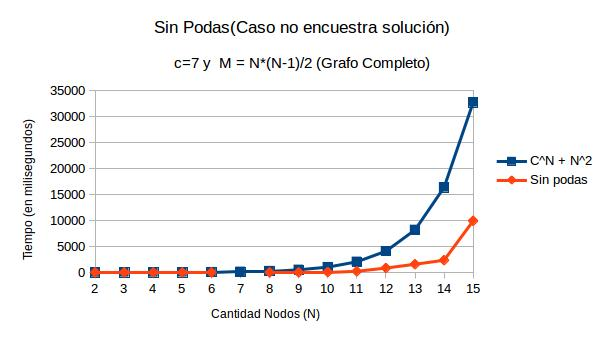
\includegraphics[scale=0.60]{imagenes/imgEjercicio2/CNESSinPodas-noSolucion.jpg}
  \end{center}
  \caption{Tiempos caso en que hay solución}
\end{figure}

 \begin{figure}
 \centering
  \subfloat[No encuentra solución]{
   \label{Fuerza brut 1}
    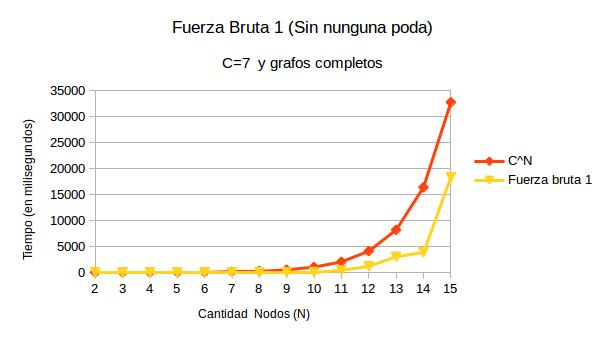
\includegraphics[width=0.55\textwidth]{imagenes/imgEjercicio2/FB1SinNingunaPoda-noSolucion.jpg}}
  \subfloat[No encuentra solucion]{
   \label{Fuerza brut 2}
    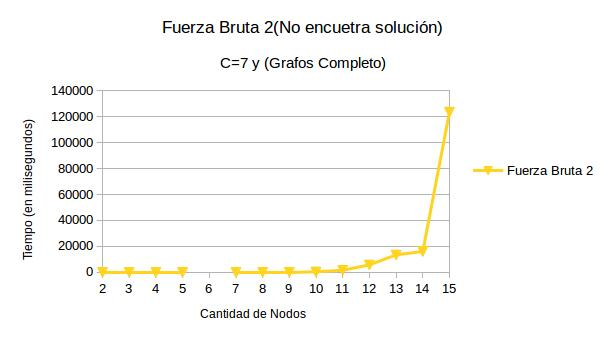
\includegraphics[width=0.55\textwidth]{imagenes/imgEjercicio2/FB2NES-noSolucion.jpg}}
 \caption{Tiempos caso en que no hay solución}
 \label{tiempos}
\end{figure}


Como vemos nuestro algoritmo tiende a comportarse exponencialmente en los graficos. 
Ahora en el siguiente grafico veremos la comparación  entre los algoritmos.


\begin{figure}[htb]
  \begin{center}
      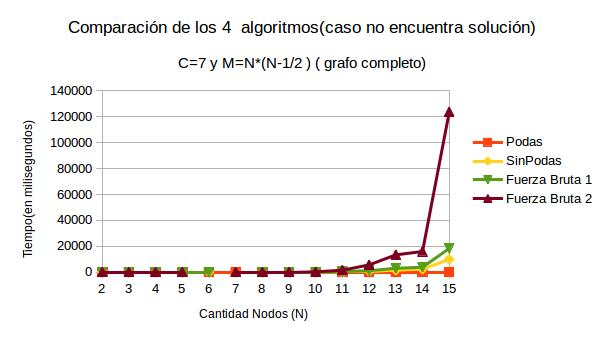
\includegraphics[scale=0.60]{imagenes/imgEjercicio2/C4ANoSolucion.jpg}
  \end{center}
  \caption{Comparacion de los tiempos}
\end{figure}


Como se ve en el grafico, los algoritmos menos eficiente son los de  \textbf{Fuerza bruta 1} y \textbf{Fuerza bruta 2} en comparación con las  versiones \textbf{Sin podas} y con \textbf{podas}. \newline
 
Cabe destacar que la version mas eficiente es la version con \textbf{Podas} como se puede apreciar en el gráfico. 


\vspace*{0.3cm}
%\textbf{completar!}


\newpage
\subsubsection{Test : Fijo N y M. Vario C}

En esta experimentación fijamos un grafo completo K12 ($N = 12$ y $M=N*(N-1)$) y variamos C. Los valores máximos que puede tomar C van desde el 2 hasta  el 10 $([0,2,..,10])$. Pintamos los grafos de manera tal que los algoritmos tengan que ejecutarse la mayor cantidad de veces(es decir tomamos instancias en caso peor). \newline

\begin{figure}[h]
  \begin{center}
      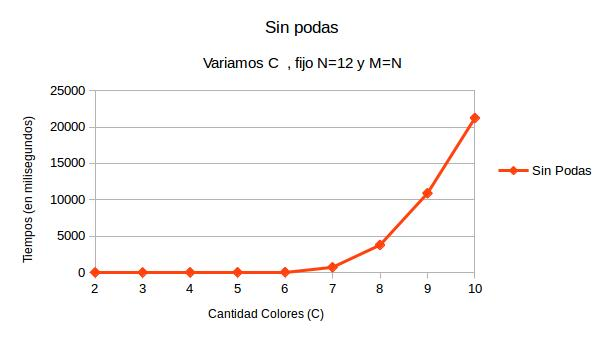
\includegraphics[scale=0.60]{imagenes/imgEjercicio2/SinPodasVariaC.jpg}
  \end{center}
  \caption{Sin podas variamos C}
\end{figure}

 \begin{figure}
 \centering
  \subfloat[No encuentra solución]{
   \label{Fuerza bruta 1}
    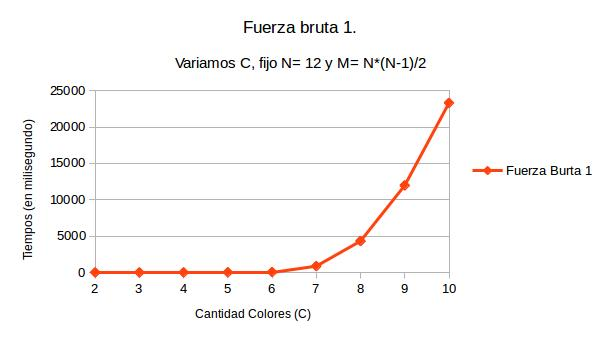
\includegraphics[width=0.55\textwidth]{imagenes/imgEjercicio2/FuerzaBruta1VariaC.jpg}}
  \subfloat[No encuentra solucion]{
   \label{Fuerza bruta 2}
    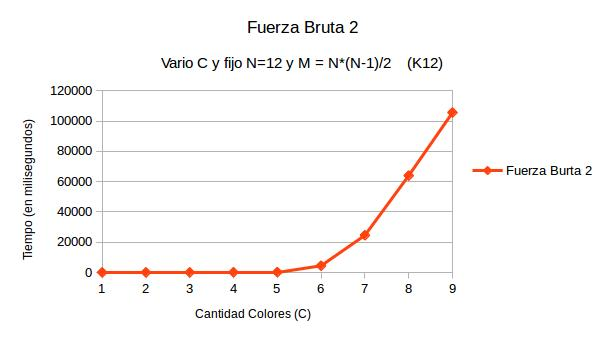
\includegraphics[width=0.55\textwidth]{imagenes/imgEjercicio2/FuerzaBruta2VariaC.jpg}}
 \caption{Furza bruta 1 y 2, variamos C}
 \label{tiempos}
\end{figure}


Como vemos ( ver figura 9 y 10) nuestro algoritmo tiende a comportarse polinomialmente en los gráficos, pues como dije mas arriba fijamos N=12 y variamos C. 
Ahora en el siguiente gráfico veremos la comparación  entre los algoritmos.

\newpage

\begin{figure}[htb]
  \begin{center}
      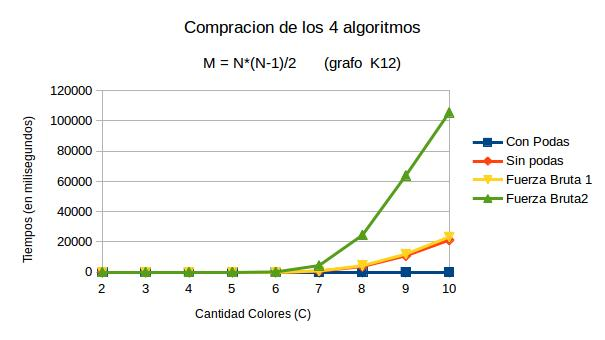
\includegraphics[scale=0.60]{imagenes/imgEjercicio2/ComparacionVariaC.jpg}
  \end{center}
  \caption{Comparacion de los tiempos}
\end{figure}


Como se puede observar en este gráfico de comparación(Figura 11), el algoritmos que se comporta mas eficientemente es el tiene las podas Y el menos eficiente es el de Fuerza bruta 2. Con esto corroboramos lo teórico con los practico a la hora de variar C. 


%En este caso lo que se va hacer es toamr una cantidad de nodos fijo, e ir variando la cantidad de colores que se puede usar.

%\vspace*{0.3cm}

%\textbf{completar!}


%\newpage
%\subsubsection{Test 3}

%\vspace*{0.3cm}

%\textbf{completar!}
